\chapter{Vergleich}
\label{cha:Vergleich}

Folgend wird zur Darstellung des Entwicklungsprozesses, und der Unterschiede zwischen der konventionellen prozeduralen Entwicklung in C/AL, und der erweiterungsbasierten Entwicklung in AL ein Beispiel in beiden Sprachen entwickelt.


\section{Aufgabenstellung}
\label{sec:Aufgabenstellung}

Für die Kunden des Auftraggebers unserer Erweiterung sollen Treuepunkte verwaltet werden. Treuepunkte werden mit dem Kauf von Waren verdient, oder von der Marketingabteilung an Bestandskunden vergeben. Treuepunkte können beim Kauf von Produkten eingelöst werden, um einen Preisnachlass zu erzielen. Eingelöste Punkte verringern den Rechnungsbetrag um einen bestimmten Geldwert, der variieren kann. So mag ein Treuepunkt im Januar 10 Cent wert sein, im Februar jedoch 15 Cent. Die Schwankung des Treuepunktwertes wird als Marketinginstrument genutzt. Auch wie viele Treuepunkte beim Einkauf vergeben werden ist variabel, so sind etwa Aktionszeiträume vorgesehen, in denen beim Einkauf doppelt so viele Treuepunkte verdient werden können.
\linebreak

Das neue Treuepunktesystem ist für das Marketing von hoher Bedeutung. So ist es erforderlich, dass Änderungen am Treuepunktekonto eines Kunden über einen Web Service an das verwendete CRM-System gemeldet werden. Für das Reporting im Unternehmen ist es außerdem nötig, dass täglich ein XML Datenträger erzeugt werden kann, in dem der Treuepunktesaldo und die Bewegungen des aktuellen Tages je Kunde ersichtlich sind. Zusätzlich zu dieser Datei für das Berichtssystem soll auch ein übersichtlicher Ausdruck in PDF-Form an die Marketingleitung gesendet werden.
\pagebreak

\section{Entwicklungsprozess}
\label{sec:Entwicklungsprozess}

\subsection{Entwicklungsumgebung}
\subsubsection{C/AL - Development Environment}
C/AL wird im \textit{Microsoft Dynamics Development Environment} entwickelt. Dabei handelt es sich eigentlich um den Client, der bis zur Version 2009 noch als Windows Client für Endbenutzer verwendet wurde, nun seit dem jedoch rein für die Entwicklung genutzt wird. Das Development Environment ist ein Windows Client, der stets sowohl mit Datenbank, als auch mit der Serverapplikation verbunden sein muss. Die Datenbankverbindung ist nötig, da darin die Applikationsobjekte gespeichert sind, die Verbindung zum Applikationsserver, um Änderungen kompilieren und ausführen zu können.
\linebreak

Das Kernstück des Development Environment bildet der \textit{Object Designer}. Der \textit{Object Designer} liefert einen Überblick über sämtliche, im System vorhanden Applikationsobjekte und Details zu Ihnen. Ein Applikationsobjekt unter C/AL wird durch eine numerische ID und seinen Namen identifiziert. Zusätzlich wird zu den einzelnen Applikationsobjekten auch gespeichert, ob und wann sie das letzte Mal geändert wurden.

\begin{figure}[h]
	\centering
	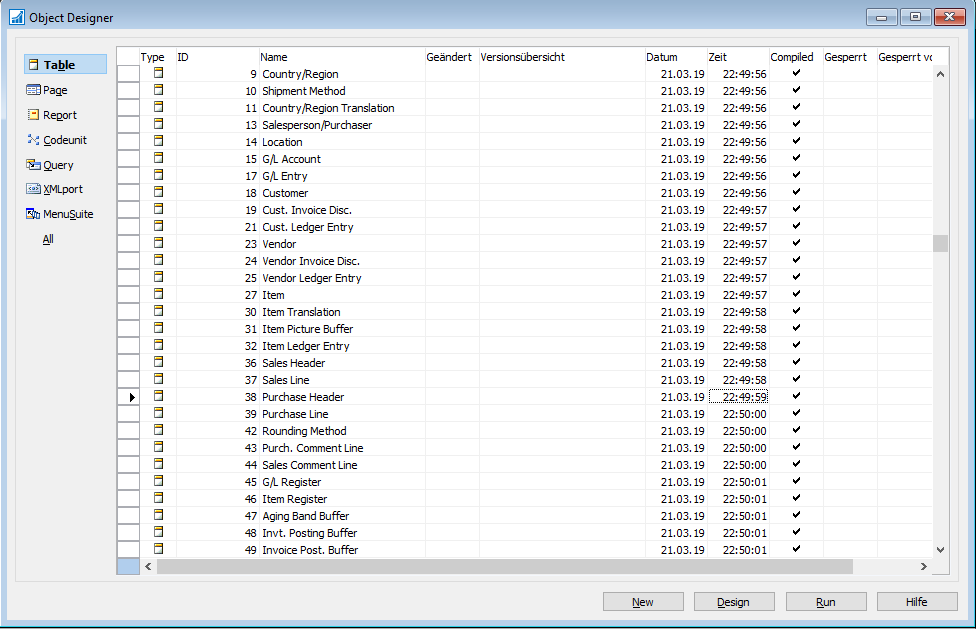
\includegraphics[width=130mm]{images/ObjectDesigner}
	\caption{Development Environment: Object Designer und C/AL Editor}
	\label{fig:ObjectDesigner}
\end{figure}

Je nach ausgewählter Objektart stellt das Development Environment einen auf die Objektart angepassten \textit{Designer} zur Verfügung, über den bereits einige Basiseinstellungen getätigt werden können. Im Falle von Tabellenobjekten, können mithilfe des Table Designers Tabellenfelder angelegt, entfernt und bearbeitet werden. Über den Designer gelangt man ebenfalls zum C/AL Editor, in dem die Implementierung der Geschäftslogik passiert.

\begin{figure}[h]
	\centering
	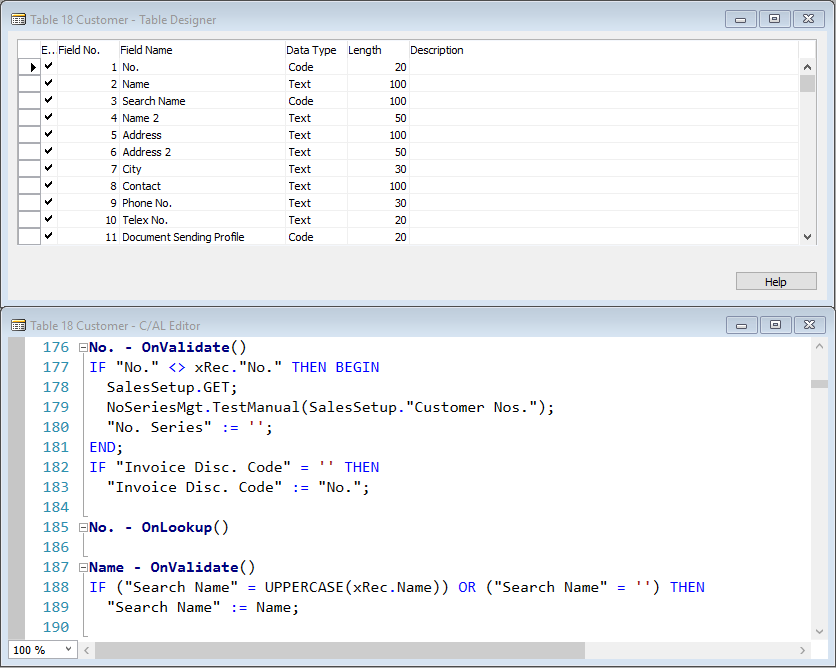
\includegraphics[width=130mm]{images/TableDesigner}
	\caption{Development Environment: Table Designer und C/AL Code Editor der Debitoren Tabelle}
	\label{fig:TableDesignerCodeEditor}
\end{figure}

Die Sprache C/AL basiert auf Pascal. Im Gegensatz zu Pascal ist C/AL jedoch rein prozedural, und rein auf die Arbeit mit Dynamics NAV bzw. Business Central spezialisiert. So bietet C/AL mithilfe der inkludierten \textit{Record API} eine einfache und effiziente Weise, Datensätze aus der Datenbank zu lesen, filtern, schreiben und zu löschen. Der Mehraufwand der in anderen Sprachen und Systemen durch die Erstellung von Datenbankverbindungen verursacht wird ist in C/AL minimal, da die Datenbankverbindung bereits durch die Verbindung zum Server gegeben ist. Der Datenbankkontext kann daher vom Applikationsserver bestimmt werden, und muss nicht im Applikationscode definiert werden. Andererseits fehlen innerhalb C/AL Funktionalitäten, die in modernen Programmiersprachen mittlerweile zum Standardumfang fehlen, wie zum Beispiel eine Möglichkeit zur Kommunikation via HTTP.
\linebreak

Um Applikationsobjekte zwischen verschiedenen Datenbanken zu transferieren, um beispielsweise entwickelte Applikationsobjekte von einem Testsystem in die Produktivumgebung zu übernehmen, bietet das Development Environment die Möglichkeit Applikationsobjekte zu exportieren. Dieser Export kann in zwei verschiedenen Formaten erfolgen. Einerseits im Textformat. Dabei werden sowohl Code als auch die im Designerfenster getätigten Einstellungen in ein spezielles Textformat gebracht. Dieses Textformat (Dateiendung .txt) ist zwar grundsätzlich durch den Menschen lesbar, definiert jedoch auch einige intern nötige Eigenschaften. Andererseits können Objekte auch im Binärformat exportiert werden (Dateiendung .fob). Das Binärformat zeichnet sich im Gegensatz zum Textformat durch geringere Dateigröße und besserer Performanz beim Importieren und Exportieren aus, und ist daher das Standardformat um Applikationsobjekte zwischen Datenbanken zu transferieren.

\subsubsection{AL - Visual Studio Code}
Die Programmierung von Erweiterungen für Microsoft Dynamics 365 Business Central erfolgt in Visual Studio Code \cite{KahlertGiza2016}. Visual Studio Code ist ein OpenSource Quelltext-Editor für verschiedenste Programmier- und Markupsprachen basierend auf dem Electron Framework. Visual Studio Code ist in der Sprache Typescript implementiert. Im Gegensatz zum Development Environment setzt Visual Studio Code kein Windows-Betriebssystem voraus, sondern kann auch unter Mac und Linux verwendet werden. Als zeitgemäße Entwicklungsumgebung liefert Visual Studio Code eine Auswahl einiger Features für Entwickler, die im Development Environment nicht vorzufinden sind. Darunter:

\begin{itemize}
	\item Refactoring Werkzeuge
	\item IntelliSense und Code-Vervollständigung
	\item Mauslose Bedienung
	\item Integrierte Source Code Verwaltung mit Git
	\item Erstellung von benutzerdefinierten Tastenkombinationen
\end{itemize}

\begin{figure}[h]
	\centering
	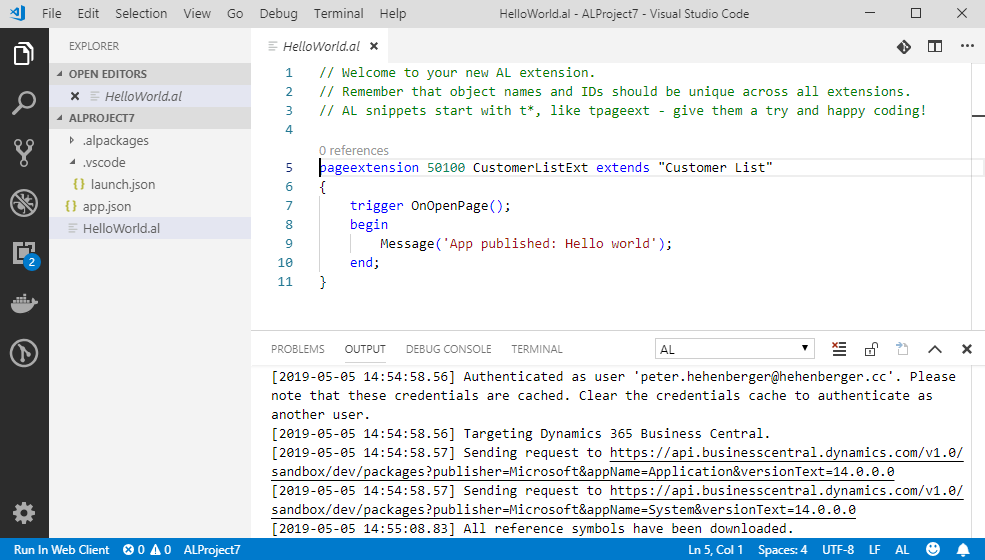
\includegraphics[width=130mm]{images/VSCode}
	\caption{Visual Studio Code: Grafische Oberfläche, Hello World Extension}
	\label{fig:VSCodeGUI}
\end{figure}

\pagebreak

Im Gegensatz zum Development Environment ist Visual Studio Code nicht dafür ausgelegt, mit Business Central und AL zu Arbeiten. Eine Basisinstallation von Visual Studio Code kann so auch nicht für die Entwicklung unter AL genutzt werden. Hier kommt jedoch eine große Stärke von Visual Studio Code ins Spiel, seine Erweiterbarkeit. Mit Business Central wird die dazugehörige Visual Studio Code Erweiterung mitgeliefert, die für die Entwicklung von AL-Erweiterungen nötig ist. Diese Erweiterung \textit{AL Language Extension}, wird im .vsix Format von Business Central zur Verfügung gestellt und lässt sich mittels weniger Klicks installieren.
\linebreak

Visual Studio Code wird monatlich automatisch mit Updates versorgt. Auch Neuheiten für die AL Spracherweiterung werden automatisch mitinstalliert, wobei es einfach möglich ist, frühere Versionen der Erweiterung zu verwenden um auch mit Systemen arbeiten zu können, die noch nicht auf dem neuesten Stand sind. Dies stellt für Entwickler einen bedeutenden Vorteil dar, da das Development Environment bei Neuerungen immer manuell geladen werden musste, und mehrere lokale Installationen nötig waren, um auch vorangegangene Versionen des Systems zu unterstützen.
\linebreak

Visual Studio Code in Kombination mit AL ist rein textbasiert. Die aus dem Development Environment bekannten verschiedenen Designer Fenster finden unter AL keine Anwendung mehr. Applikationsobjekte werden nicht mehr direkt aus der Datenbank gelesen und zurückgeschrieben, sondern existieren nun zur Entwicklungszeit als Dateien in einem Verzeichnis auf der Entwicklermaschine. Somit sind keine proprietären Exportmechanismen mehr nötig, die Datei beinhaltet sämtliche Informationen für das spätere Laufzeitobjekt, und wird als solches komplett vom Entwickler verfasst. Im Gegensatz zum Textexport aus dem Development Environment steht in den erstellten AL Dateien genau was der Entwickler vorgibt. Nicht mehr und nicht weniger. Dies ist einer der größten Vorteile, die die neue Entwicklungsumgebung mit sich bringt. Denn dadurch lässt sich der geschriebene Quellcode sinnvoll und ohne Umwege in einem Source Code Management System wie Git verwalten.


\subsection{Grundfunktionalität}
Um die Grundfunktionalität der Treuepunkterweiterung, das Sammeln und Einlösen von Treuepunkten abzubilden, sind einige Änderungen und Ergänzungen an der Standard-Tabellenstruktur von Dynamics 365 Business Central nötig. 

\pagebreak
\begin{figure}[h]
	\centering
	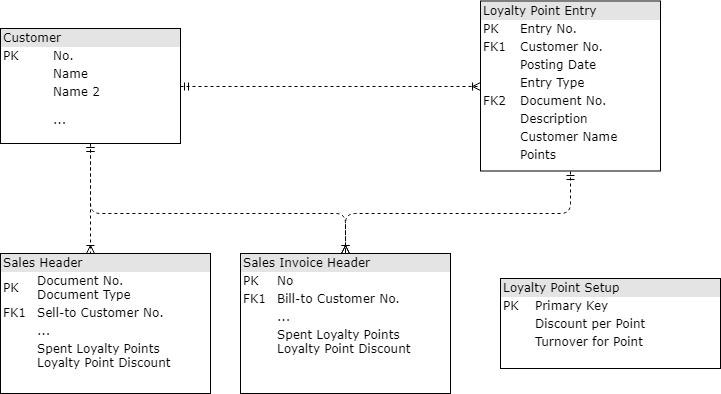
\includegraphics[width=130mm]{images/Tables}
	\caption{Grundfunktionalität: Tabellen}
	\label{fig:Tables}
\end{figure}

Es wird eine neue Tabelle \textit{Loyalty Point Entry} eingeführt, in der alle Transaktionen betreffend Treuepunkten gespeichert werden. Um diverse Auswertungen zu ermöglichen, werden neben der betroffenen Punktezahl, und dem zugehörigen Kunden auch die Dokumentennummern und die Transaktionsart (\textit{Entry Type}) gespeichert. Die Transaktionsart kann dabei einen von drei Werten annehmen: Verdienst, Einlösung und Marketing. Um die Treuepunkterweiterung konfigurierbar zu machen wird zusätzlich auch eine Setup-Tabelle \textit{Loyalty Point Entry} erstellt. Diese folgt dem in Dynamics 365 Business Central oft gebrauchten Softwaremuster der Setup-Tabelle. Dabei handelt es sich um eine Tabelle mit einem Primärschlüssel \textit{Primary Key}, in der maximal ein Datensatz gespeichert werden kann. In Tabellen dieser Art werden Konfigurationen getroffen, um andere Bereiche der Geschäftslogik zu parametrisieren.

\begin{itemize}
	\item \textit{Discount per Point}: Bestimmt für wieviele Währungseinheiten ein Treuepunkt eingelöst werden kann.
	\item \textit{Turnover for Point}: Definiert, wieviel Nettoumsatz zur Vergabe eines Treuepunktes führt.
\end{itemize}

Bei Eingabe einer neuen Verkaufsrechnung an Kunden müssen die konfigurierten Parameter abgefragt werden, um entsprechend Rechnungsrabatte zu erteilen. Wird die Rechnung danach gebucht, muss zur Behandlung der Treuepunkte in die Buchungslogik eingegriffen werden. Einerseits muss vor dem Buchen geprüft werden, ob der Kunde auch genug verfügbare Treuepunkte hat, um den Rechnungsrabatt mit seinem Punktekonto ausgleichen zu können. Diese zusätzliche Prüfung ist wichtig, da Erfassung und Verbuchung der Rechnung nicht zwangsweise zum selben Zeitpunkt erfolgen müssen. Andererseits muss nach erfolgreichem Verbuchen der Rechnung das Treuepunktekonto des Kunden angepasst werden, dabei müssen sowohl eingelöste, als auch durch die Rechnung verdiente Punkte berücksichtigt werden. Vorbereitete (\textit{ungebuchte}) Rechnungen sind Datensätze der Tabelle \textit{Sales Header}, und werden von der Buchungsroutine zu Datensätzen der Tabelle \textit{Sales Invoice Header} konvertiert. In beiden Tabellen werden die nötigen Felder zur Eingabe und Speicherung der notwendigen Daten für die Rabattvergabe hinzugefügt.

\subsubsection{C/AL}


\subsubsection{AL}

\subsection{Datenträgerexport}
\subsubsection{C/AL}
\subsubsection{AL}

\subsection{Reporting}
\subsubsection{C/AL}
\subsubsection{AL}

\subsection{Webservice-Anbindung}
\subsubsection{C/AL}
\subsubsection{AL}
















